\documentclass[11pt,a4paper]{amsart}
\ifdefined\pdftrailerid\pdftrailerid{}\fi
\usepackage[T1]{fontenc}
\usepackage{lmodern,mathtools,amssymb,booktabs,graphicx}
\usepackage[expansion=false]{microtype}
\usepackage[margin=27mm,top=25.4mm,bottom=25.4mm]{geometry}
\usepackage[hidelinks,pdfauthor={Haibo Lu},pdftitle={First-return periods on Darboux grids and hyperbolic limit cycles of polynomial fields}]{hyperref}
\newtheorem{theorem}{Theorem}[section]
\newtheorem{proposition}[theorem]{Proposition}
\newtheorem{lemma}[theorem]{Lemma}
\newtheorem{corollary}[theorem]{Corollary}
\numberwithin{equation}{section}
\newcommand{\Lu}{L_{\mathrm u}}
\newcommand{\HH}{H_{\mathrm{hyp}}}
\newcommand{\RR}{\mathbb R}
\newcommand{\CC}{\mathbb C}
\newcommand{\QQ}{\mathbb Q}
\newcommand{\W}{\mathcal W}
\newcommand{\B}{\mathcal B}
\newcommand{\A}{\mathcal A}
\newcommand{\dd}{\,d}
\newcommand{\rk}{\operatorname{rank}}
\newcommand{\sgn}{\operatorname{sgn}}
\newcommand{\Res}{\operatorname{Res}}
\newcommand{\clos}{\mathcal E}
\title[First-return periods on Darboux grids]{First-return periods on Darboux grids and hyperbolic limit cycles of polynomial fields}
\author{Haibo Lu}
\address{Shanghai Institute of Technology}
\date{}
\subjclass[2020]{34C07, 34C05, 37G15}
\keywords{Polynomial vector field, hyperbolic limit cycle, Darboux first integral, Melnikov function, Laplace transform}
\setlength{\emergencystretch}{1em}
\begin{document}
\begin{abstract}
On a rectangular grid of invariant lines, a polynomial multiplier positive throughout the bounded cells preserves their periodic orbits. Its reciprocal weights the first variation of the return map along each orbit. We compute the ranks of these first-return periods for the constant multiplier and for \(1-\kappa T_M(y)\) at generic strength \(0<\kappa<1/2\). Ordinary polynomial degree imposes a triangular cutoff on the Chebyshev indices. At any fixed transcendental anisotropy \(\lambda>1\), a dependence of periods lifts to an identity in two independent Laplace variables. Separating the two frequency indices identifies the weighted kernel even when different modes have the same horizontal pole. One polynomial perturbation realizes the resulting simple zeros as hyperbolic limit cycles on many annuli simultaneously. For every sufficiently large degree budget \(D\), the unweighted and weighted constructions give respective leading coefficients \(3/16\) and \(5/24\) in units of \(D^2(\ln D)^2/(\ln 2)^2\). The lower-order loss is explicit, and the finite-degree comparison accounts for the additional \(M\) degrees required by the multiplier.
\end{abstract}
\maketitle

\section{First-return periods at a prescribed degree}

For a perturbation \(dF-\mu\omega=0\) of a polynomial Hamiltonian, the first variation of the return map in \(F\) is the integral of \(\omega\) along the oriented regular oval~\cite[\S1, (1.1)--(1.3)]{gavrilov}. A Darboux first integral gives a related class of pseudo-Abelian periods~\cite[\S1]{firstdarboux}. We ask how many independent first-return periods can be obtained from polynomial one-forms when the unperturbed field and its perturbation must both fit in a prescribed total degree.

Let \(f(x)=T_N(x)\) and \(g(y)=T_M(y)\) be Chebyshev polynomials. Their zero lines bound heteroclinic rectangles for \(Z=(fg',-\lambda f'g)\). Inside each rectangle the level sets of \(H=-\ln(|f|^\lambda|g|)\), with \(\lambda>1\), are ovals \(\gamma_h\) for \(h=H>0\). Multiplying \(Z\) by a positive polynomial \(C\) leaves these ovals in place and changes its time element from \(dt\) to \(dt/C\). For a perturbation represented by a one-form \(\omega\), the coefficient of \(\mu\) in the return displacement is therefore \(-L_C[\omega](h)\), where \(L_C[\omega](h)=\oint_{\gamma_h}\omega/(C|fg|)\) with counterclockwise orientation, as derived in~\eqref{eq:period}.

A relatively exact form \(\omega/|fg|=dV+B\,dH\) restricts to \(dV\) on each oval. Its unweighted period vanishes when \(V\) is single-valued on the annulus. The weight changes that integral to \(\oint_{\gamma_h} C^{-1}dV=-\oint_{\gamma_h}V\,d(C^{-1})\). For \(C_0=1\) and \(C_1=1-\kappa g\), \(0<\kappa<1/2\), equation~\eqref{eq:visible} exhibits a form whose period goes from zero to strictly positive. The multiplier raises the degree from \(N+M-1\) for \(Z\) to \(N+2M-1\) for \(C_1 Z\).

Let \(\HH(D)\) be the supremum of the sizes of finite families of hyperbolic limit cycles of one real autonomous planar field \(X=(P,Q)\) with \(\max(\deg P,\deg Q)\le D\). Both degrees are ordinary total degrees in the Euclidean coordinates \(x,y\). The number of monomials is unrestricted. Hyperbolicity means that the return multiplier has modulus different from one. Counting all isolated periodic orbits gives the Hilbert number \(H(D)\ge\HH(D)\). Unmarked logarithms are natural.

\newpage
\begin{theorem}\label{th:main}
Fix \(\lambda=\pi\) and put \(c_0=3/16,\ c_1=5/24\). There are \(K>0\) and \(D_0\) such that for every integer \(D\ge D_0\) and each \(p\in\{0,1\}\) one can choose even grid orders \(N,M\ge2\) and, for \(p=1\), a strength \(\kappa\in(0,1/2)\), so that a single polynomial perturbation of \(C_pZ\) yields a field of total degree at most \(D\) with at least
\begin{equation}\label{eq:main}
 \frac{c_p D^2}{(\ln 2)^2}
       \bigl((\ln D)^2-2\ln D\ln\ln D\bigr)-K D^2\ln D
\end{equation}
distinct hyperbolic limit cycles. In particular
\(\displaystyle\liminf_{D\to\infty}\HH(D)/(D^2(\ln D)^2)\ge 5/[24(\ln 2)^2]\).
\end{theorem}

Christopher and Lloyd's fourfold construction copies existing cycles and creates new nests near centers~\cite[\S3]{christopher}. Itenberg and Shustin patchworked such examples on triangles in a subdivision of the degree polygon. Their Theorem~2.1 gives, for each integer \(d\ge3\), a field of degree \(d\) with at least \(\tfrac12 d^2\log_2 d-Kd^2\log_2(\log_2 d)\) limit cycles for an absolute \(K>0\). Their proof glues the simple cycles of the triangular pieces~\cite[Theorems 1.3.1 and 2.1, Proposition 2.2]{itenberg}. Li, Chan and Chung revised the count for symmetric Hamiltonian constructions and obtained order \(d^2\ln d\) on the sequences \(2^j-1\) and \(3\cdot2^{j-1}-1\)~\cite[\S3 and Theorem 5.2]{lichan}.

Han and Li write \(H(d)\) for the maximal number of limit cycles of a degree-\(d\) field and \(H^*(d)\) for its near-Hamiltonian counterpart. For every sufficiently small \(\epsilon>0\), their Theorem~1.3 gives \(H(d)\ge H^*(d)>(1/(2\ln2)-\epsilon)(d+2)^2\ln(d+2)\) for all sufficiently large \(d\). The recurrence propagates odd-multiplicity cycles and specified boundary tangencies on a rectangle~\cite[Theorems 1.3 and 2.1]{hanli}. Odd multiplicity can exceed one, and the final estimate counts isolated cycles. The coefficient \(1/(2\ln2)\) thus appears on the \(d^2\ln d\) scale both in the patchworking estimate and in Han and Li's lower bound for the limit inferior. In Theorem~\ref{th:main} each coordinate supplies order \(\ln D\) dyadic layers. Simple return zeros give a bound for \(\HH(D)\), hence also for \(H(D)\).

Qin and Sun use the Hamiltonian \((T_q(x)^2+\Lambda T_q(y)^2)/2\), with \(q=3^r\). We share their use of two frequency filtrations and a hierarchy of coefficients to create simple return zeros on many annuli of one field. Their ternary blocks are Cartesian products and attain full rank for sufficiently large anisotropy depending on the frequency sets~\cite[Theorems 1.1 and 2.2, Proposition 5.2]{qin}. In total vector-field degree, their hyperbolic-cycle count has leading coefficient \(1/[36(\ln3)^2]\) on the budgets \(D=4\cdot3^r-5\), \(r\ge2\), on the scale \(D^2(\ln D)^2\). Using the preceding seed at each \(D\ge31\) gives \(1/[324(\ln3)^2]\) in their Corollary~1.2. Chebyshev replication of their seeds recovers the subsequence coefficient for every sufficiently large \(D\), with the loss given in Section~\ref{sec:comparison}~\cite[Proposition 5.2]{mechanical}.

Lu's mechanical renewal constructs new nests after successive folds. Its all-degree coefficient for hyperbolic cycles is \(1/8\) in units of \((\ln2)^{-2}\), with loss \(O(D^2\ln D)\)~\cite[Theorem 1.1]{mechanical}. In these units the mechanical, unweighted-grid and weighted-grid coefficients are respectively \(6/48,9/48,10/48\). The unweighted grid gives a factor \(3/2\) over renewal and accounts for three quarters of the additive increase. The multiplier contributes the remaining \(1/48\), a further factor \(10/9\). Formula~\eqref{eq:main} gives the loss from filling the degree budgets between the dyadic squares.

At \(N=M=4\) and \(D=11\), there are 21 pairs of positive odd Chebyshev indices \((a,b)\) satisfying \(a+b\le12\). Each pair gives two perturbation forms, one in \(dx\) and one in \(dy\). At \(\lambda=\pi\), the unweighted periods of these 42 forms have rank 22. Multiplying \(Z\) by \(1-\kappa g\) raises the rank to 33 for generic \(\kappa\).
Here the unsquared factor \(T_M(y)\) enters the multiplier of a Darboux field. Total degree restricts the two frequencies to a triangle \(a+b\le D+1\), and the anisotropy can be fixed at a single transcendental value. The Laplace transform of each unweighted period samples only \((z,w)=(\lambda s,s)\). Distinct vertical frequencies can share a horizontal pole. After a common normalization the Taylor coefficients are Laurent polynomials over \(\QQ\) in the anisotropy. Transcendence lifts a putative dependence at the chosen parameter to an identity in independent \(z,w\), where Section~\ref{sec:pure} separates the frequency pairs.

To see which relations survive the multiplier, expand \(1/(1-\kappa g)\) in powers of \(\kappa g\). A polynomial family of forms with identically zero weighted period gives vanishing moments in \(g\). On one quadrant of an oval, \(g\) is a coordinate along the arc. The moments force a polynomial combination of the forms to vanish on the oval tangents, hence to be a multiple of the foliation form \(\Omega=-fg\,dH\). The other relations come from multiplying unweighted zero-period forms by \(1-\kappa g\), which uses \(M\) degrees of their allowance. Polynomial division and joint frequency separation in Section~\ref{sec:carrier} locate exactly which relations fit under the triangular cutoff.

Each frequency block and each layer of cells carries a pair of dyadic depth indices. A block indexed by \((k,l)\) is \emph{matched} to a layer indexed by \((i,j)\) when \((k,l)=(i,j)\). On that layer, its periods agree up to a cell sign. A rank \(d\) gives \(d-1\) simple zeros at positive energies, and the hierarchy of coefficients makes these zeros persist on all the selected layers in one field. Theorem~\ref{th:finite} counts the resulting hyperbolic cycles. Section~\ref{sec:comparison} compares the two grids after accounting for the additional degree of the multiplier.

\section{The grid and its first variation}\label{sec:grid}
We use $T_n(\cos t)=\cos(nt)$ and $U_{n-1}(\cos t)=\sin(nt)/\sin t$, so $T'_n=nU_{n-1}$. Set $S=D+1$. Take $N,M\ge2$ and write $C=C_p$. For $p=0$ use $C_0=1$. For $p=1$ take $C_1=1-\kappa g$, $0<\kappa<1/2$. The unweighted map is also the specialization of the weighted map at $\kappa=0$. Assume $N+(1+p)M\le S$. For a form $\omega=P_\omega\,dx+Q_\omega\,dy$ with polynomial coefficients of total degree at most $D$, consider
\begin{equation}\label{eq:field}
 X_\mu=\bigl(Cfg'-\mu Q_\omega,\;-C\lambda f'g+\mu P_\omega\bigr),\qquad
 \Omega=\lambda f'g\,dx+fg'\,dy .
\end{equation}
Since $|g|\le1$ on $[-1,1]$, the multiplier exceeds $1/2$ on the closures of the bounded cells. Both components at \(\mu=0\) have degree $d_0=N+(1+p)M-1$. Thus \eqref{eq:field} has degree at most $D$ for every real $\mu$. For fixed nonzero $\omega$ and sufficiently small nonzero $\mu$, its actual degree is $\max(d_0,\deg\omega)$. When the two degrees coincide a nonzero top coefficient of $X_0$ stays nonzero by continuity.

The $N$ roots $\cos((2a-1)\pi/(2N))$, $1\le a\le N$, and the analogous $M$ vertical-coordinate roots delimit $(N-1)(M-1)$ bounded rectangles. Between consecutive roots in each coordinate use
\begin{equation}\label{eq:chart}
 x=\cos((j\pi+\xi)/N),\qquad y=\cos((i\pi+\eta)/M),
 \qquad |\xi|,|\eta|<\pi/2 ,
\end{equation}
where $1\le j<N$, $1\le i<M$. Both coordinate derivatives are negative, so the chart preserves orientation. The lines $f=0$ and $g=0$ are invariant by \eqref{eq:field} at $\mu=0$. Their intersections are saddles with eigenvalues $Cf'g'$ and $-\lambda Cf'g'$. Along the open edge between neighboring intersections the field is nonzero and tangent to the edge. In each open cell $f=(-1)^j\cos\xi$, $g=(-1)^i\cos\eta$, and
\begin{equation}\label{eq:energy}
 H=-\lambda\ln|f|-\ln|g|=-\lambda\ln\cos\xi-\ln\cos\eta,\qquad
 \Omega=-fg\,dH .
\end{equation}
In angle coordinates $H$ has positive definite Hessian, a unique minimum at $(0,0)$ and infinite boundary values. Its positive levels are nested regular Jordan curves. We orient them counterclockwise and denote them by $\gamma_h$. At $(\xi,\eta)=(\arccos e^{-h/\lambda},0)$ the sign of $\dot\eta$ is $(-1)^{j+i}$. Hence the forward orbit traverses $(-1)^{j+i}\gamma_h$, as in Figure~\ref{fig:cells}.
\begin{figure}[tb]
\centering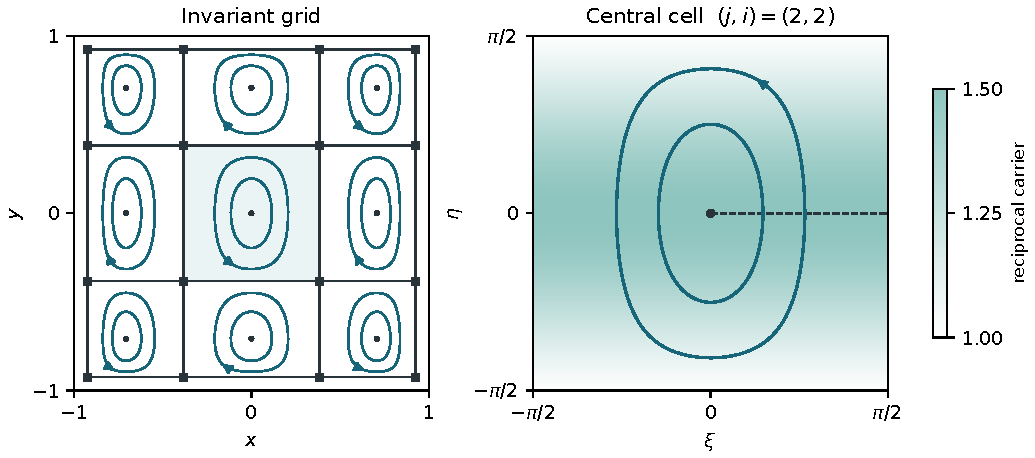
\includegraphics[width=.89\linewidth]{figures/cells.pdf}
\caption{The grid at $N=M=4$, $\lambda=\pi$. Filled squares are saddles, dots are centers and the solid curves are sampled regular levels $h=0.35,1.25$. Arrows follow the unperturbed flow on the outer ovals. At right the highlighted central cell is drawn in angle coordinates. Shading gives the extra weight $1/(1-\kappa\cos\eta)$ for $i=2$ and $\kappa=1/3$. The dashed segment is the return section.}\label{fig:cells}
\end{figure}

On a regular period annulus the time-change calculation has a simple general form. Let a smooth field $Z$ have a regular first integral $H$ there, and perturb $CZ$ by $\mu Y$ with $C>0$ and $C,Y$ smooth. Use $H$ on a transversal and let $z_h(t)$ run around the unscaled field $Z$ in time $T_Z(h)$. The coefficient of $\mu$ in the return displacement is
\[
 \int_0^{T_Z(h)}\frac{dH(Y)(z_h(t))}{C(z_h(t))}\dd t .
\]
Indeed $\dot H=\mu dH(Y)$ on the perturbed arc, and at $\mu=0$ the time element of $CZ$ is $dt/C$.

For the grid, \(Y=(-Q_\omega,P_\omega)\) gives \(dH(Y)=-\omega(Z)/(fg)\) by~\eqref{eq:energy}. Integration along the forward orbit of \(Z\) therefore gives \(-\int_{\rm forward}\omega/(C f g)\). Its orientation relative to \(\gamma_h\) is \(\sgn(fg)=(-1)^{j+i}\), so the signed factor \(fg\) becomes \(|fg|\). Use \(h=H\) on the section \(\eta=0,\ \xi>0\). On each compact interval \(I\Subset(0,\infty)\) this gives
\begin{equation}\label{eq:period}
 \mathcal P_\mu(h)-h=-\mu L_C[\omega](h)+O_{C^1(I)}(\mu^2),\qquad
 L_C[\omega](h)=\oint_{\gamma_h}\frac{\omega}{C\,|fg|}.
\end{equation}
Write \(\Lu=L_{C\equiv1}\) for the unweighted map. On the perturbed arc, \((C\Omega-\mu\omega)(X_\mu)=0\) and \(\Omega=-fg\,dH\) give the exact tangent identity \(dH=-\mu\omega/(C f g)\). To justify the remainder, enlarge \(I\) slightly inside \((0,\infty)\). The corresponding closed annular collar lies in one cell, with \(C>1/2\), \(fg\ne0\) and \(X_0\ne0\). In the chart~\eqref{eq:chart} put \(z(h)=(\arccos e^{-h/\lambda},0)\) and write \(\Phi(t,z,\mu)\) for the flow. Along one unperturbed circuit the analytic local flows compose finitely many times, so \(\Phi(t,z(h),\mu)\) is jointly real analytic near the circuit in \((t,h,\mu)\). At its return time \(T_*\) for \(h=h_*\), the equation
\[
 \eta\bigl(\Phi(t,z(h),\mu)\bigr)=0
\]
has nonzero \(t\)-derivative. The analytic implicit function theorem gives a unique return time \(T(h,\mu)\) near \(T_*\). Transversality excludes an early crossing near departure. The compact middle arc stays a positive distance from the positive half-section, and the last crossing is unique in its flow box. Thus these local times are first returns and agree on overlaps. A finite cover of \(I\) gives one range of \(\mu\) and makes \(\mathcal P_\mu(h)=H(\Phi(T(h,\mu),z(h),\mu))\) jointly analytic near \(I\times\{0\}\). Taylor expansion in \(\mu\), also after one \(h\)-derivative, gives the uniform estimate in~\eqref{eq:period}. Since \(\mathcal P_0(h)=h\), its displacement divided by \(-\mu\) extends analytically to \(\mu=0\) with value \(L_C[\omega](h)\).

One can see an individual direction become visible already at $N=M=2$. In the only cell, $f=-\cos\xi$, $g=-\cos\eta$ and $A=xy=\sin(\xi/2)\sin(\eta/2)$. Put $\omega=f\,dA+\lambda A\,df$ and $V=|f|^\lambda A$. Along the oval $\omega/|fg|=-e^h dV$, so $\Lu[\omega]=0$. With $C=1-\kappa g$, integration by parts gives
\begin{equation}\label{eq:visible}
 L_C[\omega]=\kappa e^h\oint_{\gamma_h}\frac{V\,dg}{C^2}>0\qquad (h>0).
\end{equation}
On the positive quadrant arc $V>0$ and $dg=\sin\eta\,d\eta$ is positive in the forward counterclockwise direction. Each angle reflection reverses orientation and negates the pulled-back form, so all four arcs contribute equally. The same ovals now detect a perturbation whose unweighted period vanished identically.

\subsection{Frequencies visible on a cell}
Write $2^r\mid N$, $2^s\mid M$ with $r,s\ge1$. For $1\le k\le r$, let $J_k$ consist of $1\le j<N$ of the form $2^{k-1}j'$ with $j'$ odd. Define $I_l$ in the same way for $M$. Their cardinalities are $N/2^k$ and $M/2^l$. Cells with indices divisible by $2^r$ or $2^s$, respectively, need not enter the count. Set
\[
 \A_k=(N/2^k)\{1,3,5,\ldots\},\qquad
 \B_l=(M/2^l)\{1,3,5,\ldots\},
\]
and count the pairs under the degree cutoff by
\[
 P_{kl}(X)=\#\{(a,b)\in\A_k\times\B_l:a+b\le X\}.
\]
Write $W(X)=\W_{kl}(X)$ for the span of the following two forms for every such pair,
\begin{equation}\label{eq:modes}
 E_{ab}=T_a(x)U_{b-1}(y)\,dy,\qquad F_{ab}=U_{a-1}(x)T_b(y)\,dx .
\end{equation}
Their degrees are $a+b-1$. Their leading bidegrees in each component are distinct, giving $\dim W(X)=2P_{kl}(X)$. A nonpositive threshold contributes zero.

Write $\alpha=a/N$, $\beta=b/M$, $e_l=(-1)^i$ on $I_l$ ($e_1=-1$, $e_l=1$ for $l>1$) and $\sigma=\sin(aj\pi/N)\sin(bi\pi/M)$. Reflections of either angle preserve $H$ and $C|fg|$ and reverse the orientation of its ovals. Only the part of a form odd under pullback by each reflection contributes. For $E_{ab},F_{ab}$ the resulting integrands, including the differential, are respectively
\begin{equation}\label{eq:angles}
 \frac{\sigma}{M}\frac{\sin(\alpha\xi)\cos(\beta\eta)\,d\eta}{C\cos\xi\cos\eta},\qquad
 \frac{\sigma}{N}\frac{\cos(\alpha\xi)\sin(\beta\eta)\,d\xi}{C\cos\xi\cos\eta}.
\end{equation}
Here $C_0=1$ and $C_1=1-\kappa e_l\cos\eta$. The period of a mode from $(k',l')$ vanishes on $J_k\times I_l$ if $k'<k$ or $l'<l$, since one sine factor is zero. On the matched cell layer $J_k\times I_l$ write $a=(N/2^k)u$, $b=(M/2^l)v$, $j=2^{k-1}j'$ and $i=2^{l-1}i'$. Since $aj/N=uj'/2$ and $bi/M=vi'/2$ are halves of odd integers, $\cos(aj\pi/N)=\cos(bi\pi/M)=0$. Thus \eqref{eq:angles} gives the full pullbacks pointwise, and each changes sign under either reflection. The sign
\[
 \sigma=(-1)^{(u-1)/2+(v-1)/2}\,(-1)^{(j'-1)/2+(i'-1)/2}
\]
splits into a frequency sign and a cell sign. The block period maps on its cells thus agree up to one overall sign. In computing ranks we use the cell with $j'=i'=1$.

\begin{theorem}[Block ranks]\label{th:rank}
Fix a real transcendental $\lambda>1$. Abbreviate $P=P_{kl}$. With $C=1$ the real rank of $\Lu$ on $W(X)$, for every real $X$, is
\begin{equation}\label{eq:pure}
 R_0(X)=2P(X)-P(X-N)-P(X-M).
\end{equation}
With $C=1-\kappa g$ and $N+2M\le S$, the real rank on $W(S)$ is
\begin{equation}\label{eq:carrier}
 R_1(S)=2P(S)-2P(S-N-M)-P(S-2M)+P(S-N-2M)
\end{equation}
for all $\kappa\in(0,1/2)$ outside a finite set. For fixed $N,M,S,\lambda$ one choice works for every block.
\end{theorem}
The ranks are dimensions of spaces of functions of \(h\). For instance, at \(N=M=4\), \(k=l=2\) and \(S=12\) there are 21 pairs. Equations~\eqref{eq:pure} and~\eqref{eq:carrier} give the ranks 22 and 33 quoted in the introduction.
\section{Joint Laplace separation at a fixed anisotropy}\label{sec:pure}

\subsection{A spanning set at the edge of the frequency grid}
Fix a block and suppress $k,l$. For $A=T_a(x)T_b(y)$ define
\[
 K_x(A)=f\,dA+\lambda A\,df,\qquad K_y(A)=\lambda g\,dA+A\,dg .
\]
Their unweighted periods vanish. Indeed $d(|f|^\lambda A)=|f|^\lambda K_x(A)/f$ and
$d(\lambda|g|^{1/\lambda}A)=|g|^{1/\lambda}K_y(A)/g$.
On a level $|f|^\lambda|g|=e^{-h}$ these differentials are constant multiples of $K_x(A)/|fg|$ and $K_y(A)/|fg|$.

Let $V(X)$ consist of the modes in $W(X)$ selected by their position in the array
\[
 \begin{array}{c|cc}
 &b<M&b>M\\ \hline
 a<N&E_{ab},F_{ab}&F_{ab}\\
 a>N&E_{ab}&\varnothing
 \end{array}
\]
The indices never equal $N$ or $M$. Shifts $a\mapsto a+N$ and $b\mapsto b+M$ biject their respective classes onto the indices above $N$ and $M$. Thus $|V(X)|=2P(X)-P(X-N)-P(X-M)$.

To see that $V(X)$ spans modulo the kernel, order pairs by $a+b$. If $a>N$, the coefficients of $(E_{ab},F_{ab})$ in $2K_x(T_{a-N}T_b)$ are $(b,a+(\lambda-1)N)$. All its other terms have horizontal index $|a-2N|<a$. This follows by multiplying sines and cosines, with $U_{a-1}(\cos t)\sin t=\sin(at)$. If $b>M$, the corresponding row for $2K_y(T_aT_{b-M})$ is $(M+\lambda(b-M),\lambda a)$ and the other vertical index is $|b-2M|<b$. Folded indices stay in the same block because a shift by $N$ or $M$ adds an even multiple of the elementary step. When both rows occur their determinant is
\[
 (\lambda-1)NM\{a/N-1+\lambda(1-b/M)\}\ne0
\]
for irrational $\lambda>1$. With just one row the coefficient of the omitted form is positive. Induction now gives the spanning assertion, also when $V(X)$ is empty.

\subsection{Transform and variation of the anisotropy}
The unweighted period is, up to sign in its cell, a pseudo-Abelian integral of a rational form along levels of a Darboux first integral. In the level variable $v=e^{-h}$, the Laplace transform in $h$ is the one-sided Mellin transform with measure $v^{s-1}\,dv$ on $(0,1)$. Novikov uses Mellin poles to study local uniform bounds on the zeros of pseudo-Abelian integrals for logarithmic foliations with normal crossings and admissible perturbing forms~\cite[Theorem 2 and Section 3.3]{novikov}. For the present rank question we also vary the anisotropy, which lets us distinguish two frequencies that share a Mellin pole.

Write $t>1$ for the variable anisotropy and $s$ for the complex Laplace exponent. For $\Re z>0$ put
\[
 I(z,c)=\int_{-\pi/2}^{\pi/2}(\cos\theta)^{z-1}\cos(c\theta)\dd\theta .
\]
Cauchy's beta integral gives
\begin{equation}\label{eq:beta}
 I(z,c)=\pi 2^{1-z}\Gamma(z)Y_c(z),\qquad
 Y_c(z)=\frac1{\Gamma((z+1+c)/2)\Gamma((z+1-c)/2)} .
\end{equation}
For instance, in Cauchy's integral for $(1+iu)^{-a}(1-iu)^{-b}$ put $u=\tan\theta$, $a=(z+1+c)/2$, $b=(z+1-c)/2$. The result for $\Re a,\Re b>0$, $\Re(a+b)>1$ extends to all $c$ by entirety in $c$ at fixed $z$~\cite[Eq.~5.12.8]{dlmf}.

Let $D_h$ be the angle sublevel disk $H\le h$. Green's formula applied to \eqref{eq:angles} for $E_{ab}$ gives the integral over $D_h$ of
\[
 \frac{\sigma}{M}\,\partial_\xi\!\left(\frac{\sin(\alpha\xi)}{\cos\xi}\right)
               \frac{\cos(\beta\eta)}{\cos\eta}.
\]
For $F_{ab}$ the derivative acts on $\sin(\beta\eta)/\cos\eta$ in the other variable, with prefactor $-\sigma/N$. On $\Re s>2$ the integral in $h$ against $e^{-sh}$ is absolutely convergent. Indeed, integration of its absolute majorant from $H$ to infinity gives a multiple of
$(\cos\xi)^{t\Re s-2}(\cos\eta)^{\Re s-2}$, integrable on the angle square and locally uniform in $s$. Complex powers use the real logarithm of the positive cosine. Fubini gives for $E_{ab}$ a factor $\sigma I(s,\beta)/(Ms)$ times the differentiated horizontal integral weighted by $(\cos\xi)^{ts}$. Two integrations by parts give $\alpha ts\,I(ts,\alpha)/(ts-1)$ for that integral. The endpoint factors have positive real exponent, including $(\cos\xi)^{ts-1}$. Interchanging the variables gives the second transform. With
\[
 K_t(s)=\pi^2 2^{2-ts-s}\Gamma(ts-1)\Gamma(s-1)
\]
the results divided by $K_t(s)$ are
\begin{align}
 E_{ab}:&\quad \sigma\frac{\alpha}{M}t(s-1)Y_\alpha(ts)Y_\beta(s),\nonumber\\
 F_{ab}:&\quad-\sigma\frac{\beta}{N}(ts-1)Y_\alpha(ts)Y_\beta(s).
 \label{eq:transforms}
\end{align}

At fixed $t$ these formulas sample only the line $(z,w)=(ts,s)$. To separate the two frequencies we need to vary $t$ in a putative relation, even though its coefficients at our chosen $\lambda$ are arbitrary real numbers.

\begin{lemma}\label{lem:lift}
Let the columns of a finite list be unweighted periods of block forms whose mode coefficients are Laurent polynomials in $t$ over $\QQ$. Dependence at one real transcendental value $t=\lambda>1$ implies a relation for all real $t>1$, with coefficients in $\QQ[t]$ not all zero. Under \(t=z/w,\ s=w\), the same polynomial combination of the normalized transforms in~\eqref{eq:transforms} vanishes as a meromorphic function of the independent variables \(z,w\).
\end{lemma}
\begin{proof}
Put $u=\sgn(\xi)\sqrt{-2\ln\cos\xi}$ and $v=\sgn(\eta)\sqrt{-2\ln\cos\eta}$. With the values at zero given by continuity, these are analytic coordinates and $H=(tu^2+v^2)/2$. The inverse angle $\theta(u)$ satisfies
\begin{equation}\label{eq:morse}
 \cos\theta(u)=e^{-u^2/2},\qquad
 \theta'(u)=\sqrt{u^2/(e^{u^2}-1)},\qquad \theta(0)=0 .
\end{equation}
The positive square root in~\eqref{eq:morse} is analytic and even near the origin, with rational Taylor coefficients and constant term one. Termwise integration makes the inverse angle an odd germ over \(\QQ\). In Green's formula the area density is even in each Morse coordinate. Its Taylor coefficients are rational for each normalized dyadic pair, up to the stated Laurent coefficients in $t$. Integrating a term $u^{2i}v^{2j}$ over the ellipse gives $\pi t^{-1/2}t^{-i}$ times a rational multiple of $h^{i+j+1}$. On a small ellipse the series converges uniformly, so the Taylor rows after removal of $\pi t^{-1/2}$ lie in $\QQ[t,t^{-1}]$. This requires only a neighborhood of zero for each fixed $t$. For $h>0$, rescaling the ellipse to the unit disk also gives analytic dependence on $h$ locally, by analyticity on a neighborhood of the compact disk.

If there are $d$ columns, dependence kills all $d$-rowed minors at $\lambda$. They are Laurent polynomials over \(\QQ\), hence they vanish identically by transcendence. A maximal independent set of rows over $\QQ(t)$ is finite and spans all rows, so its common nullspace contains a nonzero vector over $\QQ(t)$. Clear denominators and cancel the greatest common divisor of the entries. The resulting nonzero polynomial vector annihilates every Taylor row at every $t>1$. Convergence at zero and real-analytic uniqueness on $(0,\infty)$ give zero periods for this combination. Taking the absolutely convergent transforms first at \emph{real} $s>2$ and dividing by $K_t(s)>0$ gives an identity on the real open cone $z>w>2$. After clearing powers of $z$ and $w$ its left side is entire in $(z,w)$ because $1/\Gamma$ is entire. It vanishes everywhere by the one-variable identity theorem applied successively to the two intervals of a rectangle in the cone. Thus the uncleared identity holds wherever its original denominators do not vanish. In the frequency reduction below we replace each \(Y_c\) by a rational factor times an entire base function. These equalities hold meromorphically. A common polynomial denominator gives an entire identity, and residues are taken only in the resulting rational identities for individual base pairs.
\end{proof}

\subsection{Separating frequency pairs}
Every normalized frequency $c$ is an odd integer divided by $2^k$ or $2^l$. It has a unique representative $c_*\in(0,1)$ modulo $c\equiv\pm c_*\pmod2$. Write $Y_c(v)=B_c(v)Y_{c_*}(v)$. Then $B_{c_*}=1$ and for $m\ge1$ and $e=\pm c_*$ the gamma recurrence gives
\begin{equation}\label{eq:shift}
 B_{2m+e}(v)=\prod_{j=1}^m\frac{v+1-e-2j}{v+1+e+2(j-1)} .
\end{equation}
The zeros are positive and the poles are negative and simple. The leftmost pole is $1-c$ for $c>1$.

\begin{lemma}\label{lem:classes}
For distinct $c$ in $(0,1)$ the functions $Y_c(v)$ are independent over $\CC(v)$. Consequently the products $Y_u(z)Y_v(w)$ indexed by distinct base pairs are independent over $\CC(z,w)$.
\end{lemma}
\begin{proof}
Normalize a rational relation of shortest length so that the coefficient of $Y_b$ is one. Shift the argument by two and use $Y_c(v+2)/Y_c(v)=4/((v+1)^2-c^2)$. Eliminating $Y_b$ would shorten the relation unless every other nonzero coefficient $R$ at $Y_c$ satisfies
\[
 \frac{R(v+2)}{R(v)}=\frac{(v+1)^2-c^2}{(v+1)^2-b^2}.
\]
Sum zero and pole orders on $-1+c+2\mathbb Z$. On the left they telescope to zero, since a rational function has finite divisor there. The right side has exactly one zero and no pole in that coset because $0<b,c<1$ and $b\ne c$. A one-term relation is also impossible. For products, clear denominators so the coefficients are polynomials. Fix $z$ and apply the one-variable conclusion in $w$, then fix $w$ and apply it in $z$. Each polynomial coefficient vanishes identically.
\end{proof}

\begin{proof}[Proof of \eqref{eq:pure}]
Apply Lemma~\ref{lem:lift} to $V(X)$. By~\eqref{eq:shift} the identity takes the form
\[
 \sum_{u,v} A_{uv}(z,w)Y_u(z)Y_v(w)=0,\qquad A_{uv}\in\CC(z,w).
\] Lemma~\ref{lem:classes} gives \(A_{uv}=0\) in \(\CC(z,w)\) for each base pair. All residues below are residues of these rational coefficients. In this pair the list consists of the two modes at $(Nu,Mv)$ when present, $E$-modes with $a>N$, $b=Mv$, and $F$-modes with $a=Nu$, $b>M$. Suppose an $E$-coefficient $p(t)$ on the horizontal arm is nonzero and choose the largest such $a$. In $z$ only this term has a pole at $z_0=1-a/N<0$. Taking its residue in the rational identity over $\CC(w)$ gives a nonzero rational factor times $p(z_0/w)$. This contradicts $p\ne0$. On the vertical arm the leftmost pole in $w$ eliminates the largest $b$ in the same way, now over $\CC(z)$.

For the two remaining modes substitute $z=tw$. Absorbing the nonzero constant factors into the coefficients gives $p(t)t(w-1)+q(t)(tw-1)=0$. The linear and constant coefficients in $w$ force $p=q=0$, since $t$ is variable. This rules out dependence at $\lambda$. Together with the spanning argument it proves \eqref{eq:pure} for every threshold.
\end{proof}

\section{The weighted kernel under the triangular degree cutoff}\label{sec:carrier}

Fix $\lambda$ as in Theorem~\ref{th:rank} and one block. Let $C=1-\kappa g$. Over $\mathbb F=\RR(\kappa)$ there are two immediate sources of zero periods. A form $C\nu$ cancels the multiplier in the denominator, so any unweighted relation $\nu$ gives a weighted one. A multiple of $\Omega$ vanishes on the tangent to every oval. To identify the rank we must show that these sources exhaust the kernel \emph{within the prescribed degree}. Write $\mathcal T(X)$ for the span of $T_a(x)T_b(y)$ in the block with $a+b\le X$ and $b<M$.

A relative exactness criterion for generic Darboux centers was described by Christopher and Marde\v{s}i\'c in conference lectures~\cite{relative}. It assumes normal crossings with the line at infinity and irrational ratios of residues on distinct components. In our grid the parallel lines in one family meet at infinity and have equal residues. We work directly with the polynomial modes and their degree cutoff.

\begin{proposition}\label{prop:kernel}
Extending constant spaces to $\mathbb F$, the weighted kernel on $W(S)$ is the direct sum
\begin{equation}\label{eq:kernel}
 C\,\ker\bigl(\Lu|_{W(S-M)}\bigr)\ \oplus\ \mathcal T(S-N-M)\,\Omega .
\end{equation}
\end{proposition}

\subsection{What the moments determine}
The Taylor coefficients of $L_C$ at $h=0$ belong to $\mathbb F$. In the coordinates \eqref{eq:morse} the new factor is $(1-\kappa e_l e^{-v^2/2})^{-1}$. Writing \(q=e_l\kappa\), we have the germ
\[
 \frac{1}{1-qe^{-v^2/2}}=\frac{1}{1-q}
   \sum_{j\ge0}\left(\frac{q}{1-q}\right)^j (e^{-v^2/2}-1)^j .
\]
Only \(j\le n\) contribute to the coefficient of \(v^{2n}\), whose denominator therefore divides \((1-q)^{n+1}\). Differentiation in the Morse coordinate and multiplication by the unweighted analytic factors introduce no other parameter poles. Green's formula on the Morse ellipse therefore defines the period map into $\mathbb F[[h]]$. For each real $|\kappa|<1$ the germ converges, and analyticity in $h>0$ identifies its kernel with that of the actual integrals.

Clear denominators in a rational kernel element and write $\omega(\kappa)=\sum_{m=0}^d\kappa^m\omega_m$. Its Taylor rows vanish identically in $\kappa$, so its period is zero for all real $|\kappa|<1$ and $h>0$. Put
\[
 B=\sum_{m=0}^d g^{d-m}\omega_m .
\]
For fixed $h>0$, use $\tau=e_l\kappa$ on its oval. The uniformly convergent geometric series for $(1-\tau\cos\eta)^{-1}$ gives, at degree $d+n$ in $\tau$, the numerator
\[
 (\cos\eta)^n\sum_{m=0}^d e_l^m(\cos\eta)^{d-m}\omega_m
       = e_l^d(\cos\eta)^n B .
\]
Thus $\oint_{\gamma_h}(\cos\eta)^n B/|fg|=0$ for every $n\ge0$. Multiplication by $g=T_M$ preserves the block, since its shifts on the vertical sine and cosine indices are $b\mapsto |b\pm M|$. Consequently the \emph{full} angle pullback $F\,d\xi+G\,d\eta$ of $B/|fg|$ is odd under pullback by each reflection, by \eqref{eq:angles}. On this diagonal block the four oriented quadrant integrals agree. In particular $F(\xi,0)=G(0,\eta)=0$.

In the positive quadrant put $y_0=e^{-h}$ and $u=\cos\eta$. Then $y_0<u<1$, $\cos\xi=(y_0/u)^{1/\lambda}$. In the counterclockwise direction $u$ decreases. Reversing the integration limits gives
\begin{equation}\label{eq:moment}
 \int_{y_0}^1 u^n\left(-\frac{F}{\lambda u\tan\xi}
                      +\frac{G}{\sin\eta}\right)\dd u=0 .
\end{equation}
For fixed $h>0$ the arc and its endpoints lie inside the angle square. At $u\uparrow1$, $\tan\xi$ has a positive finite limit, $F=O(\sqrt{1-u})$, and $G/\sin\eta=O((1-u)^{-1/2})$. This last term can be unbounded. At $u\downarrow y_0$, $\tan\xi\asymp\sqrt{u-y_0}$ and $\sin\eta$ has a positive limit. The first term is $O((u-y_0)^{-1/2})$ and the second is $O(\sqrt{u-y_0})$. The bracket is integrable at both ends and continuous in the interior. Polynomial density in $C[y_0,1]$ implies that its signed measure is zero, hence that the bracket vanishes at every interior point. As $h$ varies, this says that $B$ vanishes on the oval tangents throughout the quadrant. Thus $B\wedge\Omega$ is a polynomial two-form vanishing on an open set, so it is identically zero.

The coefficients $\lambda f'g$ and $fg'$ are coprime in $\RR[x,y]$. Indeed $f,g$ have only simple roots and factors in separate variables are relatively prime. Unique factorization gives $B=B_0\Omega$ with polynomial $B_0$.

\subsection{Polynomial division and the terms above the degree cutoff}
Modulo \(C\) one has \(\kappa g\equiv1\), hence \(\omega(\kappa)\equiv\kappa^d B\). Divide \(\kappa^d B_0\) by \(C\) in \(\mathbb F[x][y]\). The divisor \(C\) has leading \(y\)-coefficient \(-2^{M-1}\kappa\). Starting with the polynomial numerator already cleared above, long division introduces only powers of \(\kappa\) in parameter denominators. These are invertible for \(0<\kappa<1/2\). It follows that
\begin{equation}\label{eq:division}
 \omega=C\nu+R\Omega,\qquad \deg_yR<M .
\end{equation}
We may take both $R$ and $\nu$ in the chosen frequency classes. To see this, expand scalars in $T_aT_b$, and the $dy,dx$ coefficients in the respective bases of \eqref{eq:modes}, allowing the free cosine index to be zero. Project each expansion to the block. The indices in $\A_k$ obey $a\equiv N/2^k\pmod{2N/2^k}$, and similarly for $\B_l$. Modulo \(2N/2^k\), the class \(N/2^k\) equals its negative, and \(N\) is a multiple of this modulus since \(k\ge1\). Thus \(a\mapsto|a\pm N|\) preserves membership and its complement. The same holds for \(b\mapsto|b\pm M|\). Products with $C$ and products of a scalar with $\Omega$ have precisely these folded shifts, by the sine and cosine products. The cosine index zero stays outside even when shifted to $N$ or $M$, and a zero sine is simply zero. This proves that the projections commute with the products in \eqref{eq:division}. The projection preserves the bound on $\deg_yR$.

For $A_{ab}=T_a(x)T_b(y)$ with $0<b<M$, set
\begin{equation}\label{eq:delta}
 D_\lambda A_{ab}=\lambda f'T_aT_b\,dx + M f T_a U_{b-1}\,dy .
\end{equation}
Here $T_a$ is evaluated at $x$, and $T_b$ and $U_{b-1}$ at $y$. The identity $T_b U_{M-1}=U_{M-b-1}+gU_{b-1}$ gives the actual quotient and remainder of $A_{ab}\Omega$ on division by $C$, namely
\begin{align}
 A_{ab}\Omega &=-\kappa^{-1}C D_\lambda A_{ab} + E(A_{ab}),\nonumber\\
 E(A_{ab})&=\kappa^{-1}\lambda f'T_aT_b\,dx+
 M f T_a\bigl(U_{M-b-1}+\kappa^{-1}U_{b-1}\bigr)\,dy .
 \label{eq:rem}
\end{align}
Both components of $E(A_{ab})$ have vertical degree below $M$. Thus $\widehat\nu=\nu-\kappa^{-1}D_\lambda R$ and $E(R)$ are the quotient and remainder of $\omega$. Per coefficient of $x^j$, univariate division by $C\in\mathbb F[y]$ lowers the degree of the quotient by at least $M$ and does not raise the degree of the remainder. Hence $\widehat\nu\in W(S-M)$, and from the $dx$ remainder $\lambda f'R/\kappa$ we get $\deg R\le S-N$.

The possible excess over the second summand in \eqref{eq:kernel} is supported on
\begin{equation}\label{eq:shell}
 \mathcal H=\{(a,b)\in\A_k\times\B_l: b<M,\quad S-N-M<a+b\le S-N\}.
\end{equation}
Decompose $R=R_{\rm low}+R_{\rm high}$ at this cutoff. Then $D_\lambda R_{\rm low}\in W(S-M)$ by \eqref{eq:delta}. Since $L_C[\omega]=\Lu[\nu]$, a nonzero $R_{\rm high}$ would yield a relation of the unweighted periods of $V(S-M)$ and of the forms $D_\lambda A_{ab}$ for $(a,b)\in\mathcal H$. Here $V(S-M)$ can replace $W(S-M)$ by its spanning property. A nonzero finite Taylor minor preserves independence of real columns after extending scalars to $\mathbb F$.

\subsection{A shared pole and its separation}
In the block of odd indices for $N=M=4$, $S=12$, the pair $(3,3)\in\mathcal H$ contributes a term at $(7,3)$. The allowed unweighted form $E_{7,1}$ in $V(8)$ has exactly the same horizontal frequency. At a fixed anisotropy both reduced transforms have the horizontal pole $s=-3/(4\lambda)$. The vertical base classes $3/4$ and $1/4$ distinguish them. Figure~\ref{fig:rank} shows the auxiliary family used to test the four high terms. Here \(W(8)\) has dimension 20 and its unweighted rank is 14, so six relations can be multiplied by \(C\). Three allowed multiples of \(\Omega\) have \(a+b\le4\). Once the four high terms have been excluded, these give all nine relations on \(W(12)\).

\begin{figure}[tb]
\centering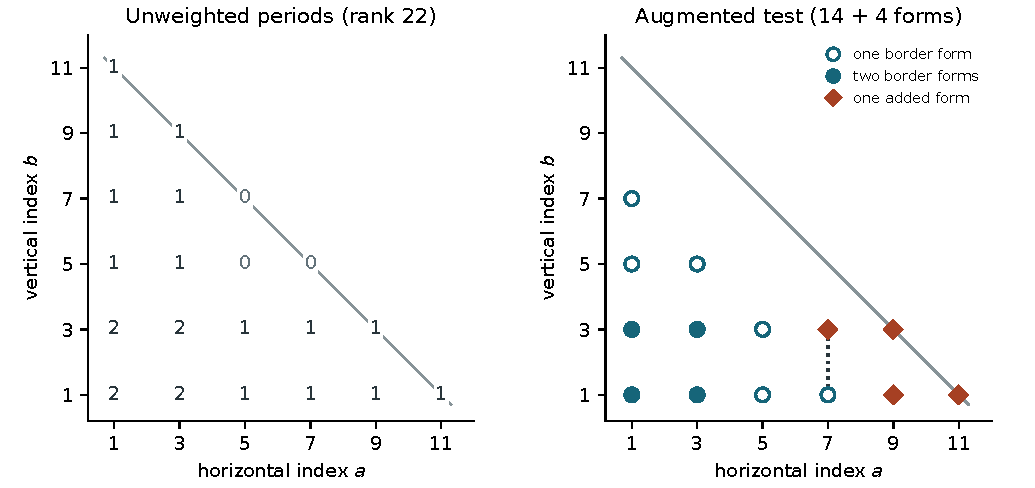
\includegraphics[width=.96\linewidth]{figures/frequencies.pdf}
\caption{Odd indices at \(N=M=4,\ D=11\). Left, the numbers count the \(E,F\) forms retained from the 42 original directions, giving unweighted rank 22. Right, six open and four filled circles represent the \(6+2\cdot4=14\) forms of \(V(8)\). Each diamond marks the upper index of one additional form \(D_\lambda A_{ab}\). The dotted segment joins two different vertical frequencies sharing horizontal index 7. Independence of these 18 forms rules out the high terms in the kernel. The full weighted rank is \(42-(6+3)=33\).}\label{fig:rank}
\end{figure}

\begin{lemma}\label{lem:shell}
The periods $\Lu[V(S-M)]$ together with $\Lu[D_\lambda A_{ab}]$ for $(a,b)\in\mathcal H$ are linearly independent at every transcendental $\lambda>1$.
\end{lemma}
\begin{proof}
Let the anisotropy vary as $t>1$. The sine and cosine products give the two horizontal indices $a+N, |a-N|$ in $D_t A_{ab}$. At the upper index the coefficients of $(E,F)$ are $(M/2,tN/2)$, and at the lower they are $(M/2,\sgn(N-a)tN/2)$. Since $a=N$ is excluded, both pairs are defined. Lemma~\ref{lem:lift} applies to this whole augmented list. In a putative polynomial relation write $q_{ab}(t)$ for the coefficient of $D_t A_{ab}$. Reduce by \eqref{eq:shift} and apply Lemma~\ref{lem:classes} to obtain a separate rational identity for \emph{each pair} of base frequencies. This step uses the open cone in $(z,w)$, including for the two summands of every $D_t A_{ab}$.

Fix a vertical index $b$ with some $q_{ab}\ne0$. Since $b<M$, it already specifies the base $v=b/M$. Among those coefficients at $b$, choose the largest horizontal index $a$. Write $A=1+a/N$, $z_0=1-A=-a/N$, and take the identity for the pair $(A_*,v)$. Consider the residue at $z=z_0$. Every ordinary term in $V(S-M)$ in this class has vertical index $b'\ge b$, hence horizontal index $a'\le S-M-b<a+N$ by the strict inequality in \eqref{eq:shell}. It cannot have this pole. Any other high term in this vertical class must have the same $b$, since all high vertical indices are below $M$. Its upper horizontal index is smaller than $a+N$, and every lower index $|a'-N|$ is strictly smaller as well. Formula \eqref{eq:shift} puts all their horizontal poles to the right of $z_0$.

The sole remaining upper term, after suppression of the common base factors, is
\[
 \sigma_{a+N,b}\,q_{ab}(z/w)\frac{z}{2w}
        \bigl[A(w-1)-v(z-1)\bigr] B_A(z) .
\]
Here $\sigma_{a+N,b}=\pm1$ is the phase of this shifted mode. For every fixed real $w>1$ all vertical rational factors are finite. The finite sum permits termwise residues, and \eqref{eq:shift} gives $\rho=\Res_{z=z_0}B_A(z)\ne0$. Its residue identity is
\begin{equation}\label{eq:residue}
 0=\sigma_{a+N,b}\,\rho\,q_{ab}(z_0/w)\frac{z_0}{2w} A(w-1+v),\qquad w>1 .
\end{equation}
All factors outside $q_{ab}$ are nonzero on this interval. As $z_0/w$ ranges over $(z_0,0)$ the polynomial $q_{ab}$ must vanish, a contradiction. Thus every high coefficient vanishes. Independence of $V(S-M)$ at a transcendental parameter then forces the remaining polynomial coefficients to vanish as well. This proves the lemma, including the case $\mathcal H=\varnothing$.
\end{proof}

\begin{proof}[Conclusion of Proposition~\ref{prop:kernel} and Theorem~\ref{th:rank}]
Lemma~\ref{lem:shell} gives $R_{\rm high}=0$. Equation \eqref{eq:division} now has $R\in\mathcal T(S-N-M)$ and $\nu\in W(S-M)$ with $\Lu[\nu]=0$. Conversely both summands in \eqref{eq:kernel} have zero weighted period and degree at most $S-1$. Their intersection is zero, since the $dx$ component of $E(R)$ is $\lambda f'R/\kappa$, which vanishes only for $R=0$.

The first summand has dimension $P(S-M-N)+P(S-2M)$ by \eqref{eq:pure}. The second has dimension $P(S-N-M)-P(S-N-2M)$ by shifting $b$ by $M$. Subtracting their sum from $2P(S)$ gives \eqref{eq:carrier}. A maximal nonzero Taylor minor over $\mathbb F$ is a rational function whose denominator has no zero in $(0,1/2)$ and whose numerator has finitely many roots. Larger minors vanish identically. At every real parameter avoiding these roots the actual germs therefore have the calculated rank. Take the union of the exceptional sets for the finitely many blocks. The two summands of~\eqref{eq:kernel} specialize into the real kernel, remain disjoint by~\eqref{eq:rem}, and have the required nullity there. For a fixed grid the complement contains rational \(\kappa\). One may even fix \(\lambda=\pi\) and one real \(\kappa\) for all integer budgets and grids, since the union of their finite exceptional sets is countable.
\end{proof}

\section{One field, integer certificates and the all-degree bound}\label{sec:counts}

\begin{theorem}[Finite grid certificate]\label{th:finite}
Let $2^r\mid N$, $2^s\mid M$, $r,s\ge1$ and $N+(1+p)M\le D+1$. Write $R_{kl}^{(p)}$ for \eqref{eq:pure} or \eqref{eq:carrier} at $S=D+1$. There exists one field \eqref{eq:field} having at least
\begin{equation}\label{eq:gridcount}
 L_p(D;N,M,r,s)=\sum_{k=1}^r\sum_{l=1}^s
       \frac{NM}{2^{k+l}}\big(R_{kl}^{(p)}-1\big)_+
\end{equation}
distinct hyperbolic limit cycles, where $x_+=\max(x,0)$.
\end{theorem}
\begin{proof}
Fix $\lambda=\pi$ and, for $p=1$, fix one $\kappa$ outside the finite union in Theorem~\ref{th:rank}. Consider a diagonal block of rank $d\ge2$. Its germs at $h=0$ have a basis with distinct orders $n_1<\cdots<n_d$, obtained by elimination. The Wronskian has leading coefficient proportional to $\prod_{i<j}(n_j-n_i)$ and is nonzero at a sufficiently small \emph{positive} point $h_0$. There the map from coefficients to the Taylor polynomial through degree $d-1$ is invertible. Prescribe the Taylor polynomial $\prod_{i=1}^{d-1}(h-h_0-\delta i)$ for $\delta>0$. The chosen coefficients stay bounded as $\delta\to0$. Rescaling $h=h_0+\delta u$ and dividing by $\delta^{d-1}$ gives $\prod_{i=1}^{d-1}(u-i)+O_{C^1}(\delta)$ for bounded $u$. This yields $d-1$ simple positive zeros, on disjoint compact intervals strictly inside the annulus. Lift the linear combination to one form $\omega_{kl}\in\W_{kl}(S)$. The common cell sign in \eqref{eq:angles} gives the same zeros on every cell of the layer. Set $\omega_{kl}=0$ if $d\le1$.

Now take $\omega=\sum_{k,l}\zeta^{k+l}\omega_{kl}$. In a cell of $J_k\times I_l$ only indices $k'\ge k$, $l'\ge l$ can contribute. After division by $\zeta^{k+l}$, the first period is the diagonal period plus $O_{C^1}(\zeta)$ on its compact intervals. With one sufficiently small $\zeta>0$ all the selected zeros persist, since there are finitely many cells and intervals. Fix this one real polynomial form. On each interval \eqref{eq:period} divided by $-\mu$ now has a simple zero $h_\mu=h_*+O(\mu)$ by the implicit function theorem. The multiplier $1-\mu L_C'[\omega](h_*)+O(\mu^2)$ is positive and different from one for small $\mu>0$. Choose disjoint compact collars around the selected ovals and take the minimum of their finitely many smallness thresholds. All these cycles belong to the same $X_\mu$ of degree at most $D$. The layer sizes give \eqref{eq:gridcount}.
\end{proof}

For a square grid $N=M=mq$, where $q=2^r$, take depth $r$ in both variables (also when $m$ is even). The following closed forms exhibit the degree cost of the carrier.
\begin{corollary}\label{cor:symmetric}
For integers $r,m\ge1$, the unweighted and weighted square grids respectively give
\begin{align}
 \HH(2mq-1)&\ge m^2\left(\tfrac34 q^2 r^2-\tfrac12 q^2+\tfrac32 q-1\right),\label{eq:sym0}\\
 \HH(3mq-1)&\ge m^2\left(\tfrac{15}{8}q^2 r^2-\tfrac14 q^2+\tfrac54 q-1\right).
 \label{eq:sym1}
\end{align}
\end{corollary}
\begin{proof}
For a nonnegative integer $j$,
\[
 P_{kl}(jN)=j^2 2^{k+l-3}+\mathbf1_{k=l}\,j2^{k-2}.
\]
Indeed the odd positive indices $u,v$ obey $u/2^k+v/2^l\le j$. For $k=l$ put $h=j2^{k-1}$ and get $h(h+1)/2$. For $k<l$, each odd $u<j2^k$ leaves $j2^{l-1}-2^{l-k-1}u$ choices for $v$. Summing over $u$ uses the fact that the first $h$ odd integers sum to $h^2$. Interchange $k,l$ for the other half. Equality along the diagonal cutoff accounts for the second term.

In \eqref{eq:pure} the combination is $2P(2N)-2P(N)$, giving $3\cdot2^{k+l-2}+\mathbf1_{k=l}2^{k-1}$. In \eqref{eq:carrier} it is $2P(3N)-3P(N)$, giving $15\cdot2^{k+l-3}+\mathbf1_{k=l}3\cdot2^{k-2}$. All ranks exceed one. Multiplying each by $N^2/2^{k+l}$ makes the main contribution constant across the $r^2$ blocks. In \eqref{eq:gridcount} the diagonal corrections sum to $N^2(1-1/q)/2$ and $3N^2(1-1/q)/4$, respectively, and subtracting one per cell costs $N^2(1-1/q)^2$. This yields the two formulas.
\end{proof}

In these two grids the leading contributions per $(D+1)^2r^2$ are $(3/4)/2^2=3/16$ and $(15/8)/3^2=5/24$. Thus the additional rank pays for the extra $M$ degrees of the carrier even after both counts are expressed in the final degree.

\begin{proof}[Proof of Theorem~\ref{th:main}]
For $S=D+1\ge16$, let $b=1+\lfloor\log_2 S\rfloor$ be its binary length. Choose $q$ as the largest power of two with $bq\le S$, and put $m=\lfloor S/(3q)\rfloor$. These integer operations give an explicit witness at every such budget. Since $S/(2b)<q\le S/b$, we have $m\ge1$, $r=\log_2 q\ge1$, $3mq-1\le D$, and
\[
 N=mq=S/3+O(S/\ln S),\qquad
 r=(\ln S-\ln\ln S)/\ln2+O(1).
\]
The right side of \eqref{eq:sym1} is $(15/8)N^2 r^2+O(S^2)$. In $N^2$ the rounding error $O(S^2/\ln S)$ costs $O(S^2\ln S)$ after multiplication. Squaring $r$ gives $[(\ln S)^2-2\ln S\ln\ln S]/(\ln 2)^2+O(\ln S)$, since $(\ln\ln S)^2=O(\ln S)$. Substitution, $(15/8)/9=5/24$ and $S=D+1$ give \eqref{eq:main}. The witness uses the budget $3mq-1$ even when the prescribed degree is between grid degrees.
\end{proof}

\subsection{Comparison at the same degree}
For $q=3^r$, $r\ge2$, Qin and Sun's Theorem~1.1 produces $4r^2q^2/9-(q-1)^2$ hyperbolic cycles at degree at most $4q-5$. The Hamiltonian has degree $2q$ and the perturbation sets the final cost. Substitution of the final degree gives coefficient $1/[36(\ln3)^2]$ along the subsequence. Their Corollary~1.2 uses monotonicity between successive seeds, giving $1/[324(\ln3)^2]$ for every $D\ge31$, with a loss of order $D^2\ln D$ relative to that leading term~\cite[Theorem 1.1, Corollary 1.2 and Section 6]{qin}.

The Chebyshev replication of Eshkobilov, Kadyrov and Mamayusupov copies $L$ cycles of degree $d$ to $m^2L$ cycles at degree at most $m(d+1)-1$~\cite[Theorem 1]{replication}. Each branch is a local orbital equivalence, so the multiplier is preserved or inverted. Applied to the ternary seeds, this recovers the subsequence coefficient for all sufficiently large $D$, with the same logarithmic rounding term as in \eqref{eq:main}. Lu's Proposition~5.2 gives this combination explicitly. The mechanical theorem gives the larger coefficient $1/[8(\ln2)^2]$ with loss $O(D^2\ln D)$. Thus the comparisons involve both the degree quantifier and the precision below the leading term~\cite[Theorem 1.1 and Proposition 5.2]{mechanical}.

For a finite comparison, let $G(D)$ be the maximum of \eqref{eq:gridcount} over the two carrier choices and admissible even $N,M$, using their full binary depths. Shorter depths only omit nonnegative summands. The four comparison families in Table~\ref{tab:finite} are those specified in Lu's finite-degree supplement~\cite[Sections 1--3]{supplement}. Its common copy and unused-degree rule takes a seed ledger $b$ to $\clos[b](D)=\max_{d\le D}b(d)\lfloor(D+1)/(d+1)\rfloor^2$. The classical column uses its four-root Han--Li tree and listed direct seeds, the two-source column starts empty, the ternary column uses the seeds above, and the mechanical column starts from the binary-prefix renewal of~\cite[Proposition 3.3]{mechanical}. The classical ledger records bounds for $H$ as stated there. The other columns count hyperbolic cycles.

\begin{table}[tb]
\caption{Finite certificates at total degree at most $D$. The triple is one maximizing $(p,N,M)$ for the grid. A dash means that the ternary ledger has no seed at that degree.}\label{tab:finite}
\centering\small
\begin{tabular}{r r l r r r r}
\toprule
 $D$&$G(D)$&$(p,N,M)$&Classical&Two-source&Ternary&Mechanical\\
\midrule
3&3&$(0,2,2)$&13&0&---&0\\
5&11&$(0,2,4)$&37&0&---&4\\
7&45&$(0,4,4)$&74&0&---&20\\
11&140&$(0,4,8)$&153&80&---&72\\
23&1,161&$(0,8,16)$&833&440&---&676\\
31&2,967&$(0,16,16)$&1,801&1,320&80&1,940\\
63&18,735&$(0,32,32)$&9,065&7,912&320&12,756\\
95&48,071&$(0,32,64)$&21,705&20,648&720&30,676\\
191&275,535&$(1,64,64)$&104,681&114,152&2,880&176,724\\
319&875,631&$(1,64,128)$&280,073&394,472&40,256&652,116\\
\bottomrule
\end{tabular}
\end{table}

At $D=5$, the symmetric weighted certificate gives eight cycles and the rectangular unweighted one gives eleven. The mechanical recurrence has half-degree three, prefixes $1,3$ and one birth contribution $4(3-1-1)=4$. The published reversible-center construction already gives $H(5)\ge37$~\cite{reversible}. At $D=11$ the classical ledger likewise exceeds the grid. On the finite range $5\le D\le350$, direct enumeration gives $G(D)>\clos[b_{\rm mech}](D)$ at each of the 346 degrees. These comparisons refer to the specified ledgers.

The verification files enumerate these integer bounds, reconstruct Taylor matrices at rational sample parameters and check the frequency collisions in Lemma~\ref{lem:shell}. The proof of Theorem~\ref{th:rank} determines the dimension for arbitrary admissible sizes. Its scope is the two displayed carriers and the stated blocks. Optimality among general positive polynomial multipliers and a further logarithmic factor lie outside these conclusions.

\section{Comparisons at the same total degree}\label{sec:comparison}

\subsection{Subsequences and all-degree estimates}
With \(q=3^r\), \(r\ge2\), Qin and Sun's Theorem~1.1 gives the hyperbolic-cycle seeds
\begin{equation}\label{eq:ternary}
 d_r=4q-5,\qquad b_Q(d_r)=4r^2q^2/9-(q-1)^2 .
\end{equation}
The Hamiltonian has degree \(2q\), and the perturbed field has degree at most \(d_r\). Substituting \(r=\ln q/\ln3\) in~\eqref{eq:ternary} gives the coefficient \(1/[36(\ln3)^2]\) of \(d_r^2(\ln d_r)^2\). At each \(D\ge31\), taking the largest \(d_r\le D\) gives the monotonicity bound of Corollary~1.2, with coefficient \(1/[324(\ln3)^2]\) and loss \(O(D^2\ln D)\). The same hyperbolic cycles witness that bound~\cite[Theorem 1.1, Corollary 1.2 and \S6]{qin}.

For a finite family of \(L\) cycles at degree \(d\), the Chebyshev pullback of Eshkobilov, Kadyrov and Mamayusupov gives \(m^2L\) cycles at degree at most \(m(d+1)-1\)~\cite[Theorem 1]{replication}. Indeed, after affine localization, \((T_m(x),T_m(y))\) maps each branch rectangle diffeomorphically onto the same square. Multiplying the two pulled-back components \(P(T_m(x),T_m(y)),Q(T_m(x),T_m(y))\) by \(T'_m(y),T'_m(x)\), respectively, gives the stated degree and a time change of constant sign on each branch. The return map is conjugate to the original or its inverse, so this operation also preserves hyperbolicity. Applying it to~\eqref{eq:ternary} with \(q\asymp D/\ln D\) recovers the coefficient \(1/[36(\ln3)^2]\) at every sufficiently large degree with the \(-2\ln D\ln\ln D\) correction, as shown in Lu's Proposition~5.2~\cite{mechanical}. The mechanical preprint's Theorem~1.1 obtains \(1/[8(\ln2)^2]\) at every sufficiently large degree with loss \(O(D^2\ln D)\). These results and Theorem~\ref{th:main} all count hyperbolic cycles of real autonomous polynomial fields.

\subsection{Finite grid counts}
For \(p=0,1\) let \(G_p(D)\) be the maximum of~\eqref{eq:gridcount} over admissible even \(N,M\) for this \(p\). Use full dyadic depths \(r=\nu_2(N),s=\nu_2(M)\), since shorter depths omit nonnegative summands. The unweighted family starts at \(D=3\), the weighted family at \(D=5\).

For comparison families with seed bounds \(b(d)\), write
\[
 \clos[b](D)=\max_{d\le D}b(d)\left\lfloor\frac{D+1}{d+1}\right\rfloor^2 .
\]
This permits both replication and unused degree. Each grid family already includes this rule. Indeed scaling \(N,M\) by \(m\) and \(S\) by \(m\) scales both frequency sets at the original depths by \(m\). All ranks at those depths are identical, and each layer has \(m^2\) times as many cells. Any additional depths add nonnegative terms. For two nested budgets one may choose the same \(\kappa\) outside both finite exceptional sets, so enlarging \(D\) can only increase or preserve each rank. Thus \(\clos[G_p]=G_p\) wherever the family is available.

Table~\ref{tab:finite} gives the two grid counts against the four families of Lu's finite-degree supplement~\cite[\S\S1--3]{supplement}. Each comparison column applies \(\clos\) to the following seeds.

\begin{table}[htbp]
\caption{Constructive lower bounds at the same total degree budget \(D\). The two grids are optimized separately. The last four columns use the specified tree and direct seeds, empty-seed two-source renewal, ternary seeds and mechanical renewal, each with replication and unused degree allowed. The classical column bounds \(H(D)\) from below. The other columns bound \(\HH(D)\) from below. A dash means that no seed fits.}\label{tab:finite}
\centering\small
\begin{tabular}{r rr rrrr}
\toprule
 \(D\)&\(G_0(D)\)&\(G_1(D)\)&Classical&Two-source&Ternary&Mechanical\\
\midrule
3&3&---&13&0&---&0\\
5&11&8&37&0&---&4\\
11&140&120&153&80&---&72\\
23&1,161&1,073&833&440&---&676\\
31&2,967&2,495&1,801&1,320&80&1,940\\
78&24,399&20,799&10,358&12,664&320&17,420\\
79&24,879&25,947&12,545&13,512&320&20,308\\
95&48,071&47,783&21,705&20,648&720&30,676\\
191&271,503&275,535&104,681&114,152&2,880&176,724\\
255&594,111&561,279&208,297&236,904&8,960&415,572\\
319&793,839&875,631&280,073&394,472&40,256&652,116\\
\bottomrule
\end{tabular}
\end{table}

\smallskip\noindent\emph{Classical.}
Han and Li's hypothesis \(H(d,r,L)\) requires a degree-\(d\) field with property \(T(r)\) and \(L\) odd-multiplicity cycles on a rectangle. Begin with
\((3,1,13),(4,1,20),(5,2,28),(6,2,35)\).
The children have degrees \(2d+1,2d+2\), common index \(2r+1\), and counts \(4L+(4r+1)d-2r,\ 4L+(4r+1)d\), respectively~\cite[Lemma 2.7 and Theorem 2.1]{hanli}. Take the larger of the native tree count and the direct seed at each degree. The direct seeds include the classical \(H(2)\ge4\) recalled in~\cite[\S2]{reversible}. Theorem~1 of Prohens and Torregrosa gives \(28,37,53,74,96,120,142\) at \(d=4,\ldots,10\). Their bounds \(212,384,568,1184,1536,1920,2272\) at \(d=13,17,21,31,35,39,43\) appear in Corollary~2(a) of the UAB accepted manuscript, numbered Theorem~2(a) in the journal~\cite{reversible}. Only the four property-\(T\) states and their descendants feed the tree.

\smallskip\noindent\emph{Two-source and ternary.}
For \(u\ge3\), Lu's renewal takes a field of degree at most \(u\) with \(L\) selected hyperbolic cycles to one of degree at most \(2u+5\) with \(4L+4(u+2)(u+1)\) selected hyperbolic cycles~\cite[Proposition 4.1 and \S4.3]{twosource}. The binary construction in this column starts with \(b_T(d)=0\) for \(3\le d\le10\), then uses \(b_T(d)=4b_T(u)+4(u+2)(u+1)\) for \(u=\lfloor(d-5)/2\rfloor\) and \(d\ge11\). The theorem also permits a nonempty hyperbolic seed. Such an input contributes \(4L\) old cycles at the first renewal and defines a different sequence. The ternary seeds are exactly~\eqref{eq:ternary}.

\smallskip\noindent\emph{Mechanical.}
Set \(b_M(d)=B(\lfloor(d+1)/2\rfloor)\), where \(B(1)=0\). With \(u\ge2\), \(j=\lfloor\log_2u\rfloor\) and \(h_k=\lfloor u/2^{k+1}\rfloor\), Lu's binary-prefix recurrence~\cite[Proposition 3.3]{mechanical} gives
\[
 B(u)=4B(\lfloor u/2\rfloor)
     +4\sum_{k=0}^{j-1}2^k\bigl[h_k(u-2^kh_k)-1\bigr].
\]
In particular \(B(3)=4\), the entry at \(D=5\).

At \(D=5\) the \(2\times4\) unweighted grid gives eleven cycles and the \(2\times2\) weighted grid gives eight, while the reversible-center construction gives \(H(5)\ge37\)~\cite[Theorem 1]{reversible}. Table~\ref{tab:order} gives the full comparison on the common grid domain \(5\le D\le350\). Even the larger of \(G_0(D),G_1(D)\) falls below the classical count at the nine budgets \(5,\ldots,11,13,14\). It exceeds each available entry of the four specified comparison families at every other budget in this interval.

\begin{table}[htbp]
\caption{Exact ordering against the four specified constructions for \(5\le D\le350\). Intervals denote integer budgets. Each grid strictly exceeds the comparison bound \(B(D)\) at every other degree in that row's domain. There are no ties.}\label{tab:order}
\centering\small
\begin{tabular}{@{}lccc@{}}
\toprule
Bound \(B\)&Domain of comparison&\(G_0(D)<B(D)\)&\(G_1(D)<B(D)\)\\
\midrule
Classical&\([5,350]\)&\([5,11]\cup[13,14]\)&\([5,19]\cup\{21\}\)\\
Two-source (empty seed)&\([5,350]\)&\(\varnothing\)&\(\varnothing\)\\
Ternary&\([31,350]\)&\(\varnothing\)&\(\varnothing\)\\
Mechanical&\([5,350]\)&\(\varnothing\)&\(\varnothing\)\\
\bottomrule
\end{tabular}
\end{table}

On \(5\le D\le350\), the weighted count is strictly larger than the unweighted count at exactly 95 budgets,
\[
 D\in [79,94]\cup[159,205]\cup[319,350].
\]
The unweighted count is strictly larger on \([5,78]\cup[95,158]\cup[206,318]\), the remaining 251 budgets. At \(D=79\) the weighted \(16\times32\) grid gives \(25{,}947\) cycles and the unweighted \(32\times32\) grid gives \(24{,}879\). At \(D=255\) the unweighted \(128\times128\) square gives \(594{,}111\). Multiplying the unperturbed field of that square by \(1-\kappa T_{128}(y)\) would raise its degree to 383. The maximizing weighted rectangle at this budget is \(128\times64\), with \(561{,}279\) cycles.

The coefficient \(5/24\) in Theorem~\ref{th:main} comes from fitting weighted squares into every sufficiently large budget. The finite ordering depends on which integer grid orders fit each \(D\). The tables give lower bounds from six specified constructions, while the Hilbert numbers allow every polynomial field at the given budget. The accompanying \path{verification/results/degrees.csv} gives a maximizing pair \((N,M)\) for each available grid family at every budget \(3\le D\le350\).

\bibliographystyle{amsplain}
\bibliography{references}
\end{document}
